\section{Design and Methodology}

\subsection{Data Collection}
The data was collected using the Twitter Streaming API \footnote{\url{https://developer.twitter.com}} between October 2017 and September 2018. The Streaming API allows you to stream real-time tweets. A location filter was specified so that only tweets posted from within the bounding box of Dublin were returned (Figure ~\ref{fig:dublinBB}). A total of 2.5 million tweets were collected.

After inspecting the collection of tweets it was found that although a bounding box had been specified, not all tweets in the collection had been posted from Dublin. A significant amount of tweets had slipped through Twitter's location filter. This meant that the first step required was to filter the dataset to ensure, as much as was possible, that all tweets related to Dublin.

\subsection{Data Filtering}
The raw dataset was cleaned and filtered, so that it only contained English language tweets posted from Dublin, and secondly so that it only contained tweets mentioning hotels.

\subsubsection{Filtering Out Non-Dublin Tweets}
All of the tweets in the dataset were Geo-tagged because they were collected with Twitter's location filter. This meant they all had location data: a specified location from which the tweet was posted. There are two types of Geo-tagged tweets, tweets with a 'Point Coordinate', a specific latitude/longitude or point coordinate, and tweets with a 'Twitter Place', a specified bounding box defining a certain place.

Only 7.23\% of the tweets in the collection had point coordinates so a combination of the Twitter place and the point coordinates was used to filter out any non-Dublin tweets that had ended up in the dataset. A bounding box for the Dublin area was defined (North Latitude: 53.425210, South Latitude: 53.223430, East Longitude: -6.043924, West Longitude: -6.447485). Tweets with a point coordinate and tweets with only a Twitter place were filtered differently. Each tweet with a point coordinate was checked to see if the point coordinate fell within the defined bounding box for Dublin. If it lay inside the box it was kept, otherwise, it was filtered out. Each tweet with a Twitter place has a bounding box specifying the location of the place. The centroid of this bounding box was calculated for each tweet. Then the centroid was checked to see if it fell within the defined bounding box for Dublin. If it lay inside the box it was kept, otherwise, it was filtered out. 

The filtered dataset consisted of 1.6 million tweets posted from Dublin between October 2017 and September 2018.

\subsubsection{Filtering Tweets About Hotels}
A list of the hotels in Dublin was compiled. This included the hotel's name and the hotel's Twitter handles (@hotelname). This list consisted of 159 hotels and Twitter handles.

The tweets were stored in a Lucene index. A fuzzy search query was used to match the tweets against each of the hotel names and hotel Twitter handles. The fuzzy search query uses a similarity measure that is based on the Damerau-Levenshtein algorithm. The maximum edits option was set to two, meaning that strings with a maximum difference of two characters would still match. This accounted for misspellings and broadened our search slightly. We experimented with higher numbers of maximum edits but found that too many irrelevant tweets were returned.

No NLP (natural language processing) technique that attempts to identify all mentions will be 100\% accurate. Users will refer to hotels in all manner of ways, anaphora like 'the hotel'. We have tried to be reasonably conservative and ensure we have a pretty clean dataset, but there are a range of ways to identify hotels that could be experimented with. 

This further filtered dataset consisted of 3115 tweets that mention hotels posted from Dublin between October 2017 and September 2018.

\subsection{Dataset Annotation}

In order to train a classifier to categorise tweets as review-like tweets, as tweets that contain some content and as irrelevant tweets, a set of tweets had to first be manually annotated. The set of 3115 tweets about hotels in Dublin was annotated. This involved building an annotation webpage where users could view tweets and assign them labels.

A simple webpage was created in order to annotate the tweets (Figure ~\ref{fig:webpage}). 

\begin{figure}[h!]
\centering
\fbox{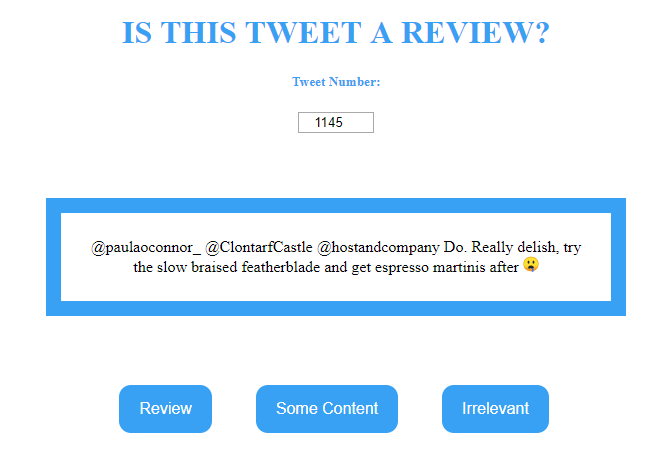
\includegraphics[width=0.95\columnwidth]{design_and_methodology/webpage.PNG}}
\caption{\label{fig:webpage} Tweet Annotation Webpage.}
\end{figure}

The text of each tweet was displayed alongside three buttons: 'Review', 'Some Content' and 'Irrelevant'. The participant could click on the option that they thought best described the tweet shown. Once they chose a label, the next tweet would be displayed. 

The following instructions, describing what a 'Review', 'Some Content' and 'Irrelevant' tweet should look like accompanied the webpage:
\begin{itemize}
    \item Review: The tweet could be considered as a review (of any aspects related to a hotel such as the venue, food, view, swimming pool, etc.) for any hotel. Examples would include: \emph{"Amazing view of the Aviva Stadium from my hotel balcony at hotel X"} (positive review), "Room service was awful at hotel Y" (negative review), \emph{"Thank you hotel X for a lovely stay"} (positive review) or \emph{"Had an awful night at hotel Y"} (negative review).
    \item Some Content: The tweet doesn't look like a review, but it does provide some information related to a hotel, such as the hotel hosts events, information on the menu, information related to accommodation, etc. Examples would include: \emph{"Hotel Z serves Tuna salad on Wednesday”} or \emph{“A packed room for the 2018 fashion conference at Hotel X”}.
    \item Irrelevant: This tweet is completely irrelevant. While perhaps mentioning the name of a hotel, the tweet doesn't give any additional information about that hotel or offer any opinions related to the hotel.
\end{itemize}

In this research, we decided to focus solely on the text of the tweets. For this reason, all images, videos and URLs were stripped from the tweets before being displayed on the annotation webpage. Images, videos and URLs could all carry valuable information and could be considered in future research. 

The annotation webpage was circulated to friends, family and members of the Adapt Research Centre to gather annotations.

\subsection{Tweet Classification}
The annotated set of tweets was used to train a series of different classifiers with different feature representations to determine which combination was most suited to the task. These classifiers were implemented using Python's Scikit Learn library \cite{scikit-learn}. The data was split into a training set and a testing set. The data was split 80:20 where 80\% was used for training and 20\% was used for testing.

\subsubsection{Data Pre-processing}

The following steps were taken to pre-process the tweets before they were used to train the classifiers:
\begin{itemize}
    \item Emojis: Emojis were removed and replaced with text using Python's Emoji library \cite{emoji}.
    \item Punctuation: The majority of special characters and punctuation was removed from the tweets. This included everything except the digits 0 - 9, the letters a - z (in upper and lower case), and the following set of symbols: . , ? ! ( ) \& ' - . 
    \item Single Characters: All single characters were removed.
    \item Case Change: Words were split on case changes. For example \emph{'MerrionHotel'} --> \emph{'Merrion Hotel'}.
    \item Word-digit Boundaries: Words were split on word-digit boundaries. For example \emph{'HouseDublin2'} --> \emph{'House Dublin 2'}.
    \item Lowercase: All text was converted to lower case.
    \item Stemming: Stemming was performed using the Word Net Lemmatizer from the Natural Language Toolkit \footnote{\url{https://www.nltk.org/}}.
    \item Stop Words: Stop words were removed in some cases using Scikit Learn's Engligh stop word list. It will be clearly stated in all cases where stop words were removed.
\end{itemize}

\subsubsection{Feature Representation}

We experimented with seven different feature extraction methods to see which performed best at classifying the Twitter data. Tweets are short with a maximum of 280 characters, which has led to the use of particular characteristic features, such as, hashtags, emojis, Twitter handles, URLs, images, videos and gifs, which don't occur in standard text. This means that standard feature extraction methods that perform well on regular, long-form text will not necessarily perform well on Twitter data.

The seven feature extraction methods implemented were:
\begin{itemize}
    \item Unigram Bag-of-Words (BOW): A unigram implementation of BOW using Scikit Learn's Count Vectorizer. In Bag-of-Words (BOW) documents are described by word occurrences. Each tweet is then represented as a feature vector consisting of ones and zeroes. One representing a term's occurrence and zero representing a term's absence.
    \item Unigram TF-IDF: A unigram implementation of TF-IDF using Scikit Learn's Count Vectorizer and TF-IDF transformer. BOW can be extended with TF-IDF (Term Frequency - Inverse Document Frequency). Term frequency is the frequency of the word in the current document. Inverse Document Frequency takes into account how often the word occurs in the whole dataset. The idea is to balance how important a term is in a document versus how important it is in the entire collection. The TF-IDF score is used to re-weight the count features produced by the Count Vectorizer.
    \item Bigram TF-IDF: A bigram implementation of TF-IDF using Scikit Learn's Count Vectorizer and TF-IDF transformer. Another extension of BOW is the use of N-grams. N-grams help to address the problem BOW has with discarding word order. An N-gram is a sequence of N consecutive terms. Combining bigrams with BOW means that occurrences of pairs of consecutive words are counted instead of individual terms.
    \item Trigram TF-IDF: A trigram implementation of TF-IDF using Scikit Learn's Count Vectorizer and TF-IDF transformer.
    \item Unigram TF-IDF (stop words removed): A unigram implementation of TF-IDF with stop words removed using Scikit Learn's Count Vectorizer, TF-IDF transformer and English stop word list.
    \item Word2Vec: Gensim's implementation of word2vec with Google's pretrained model. Word2Vec takes a dataset as its input and produces a vector space. Each word in the dataset is represented by a corresponding vector. It groups the vector of similar words together in the vector space. Cosine similarity, the cosine of the angle between two vectors, measures the similarity of vectors in the vector space.    
    \item Doc2Vec: Gensim's implementation of doc2vec, each tweet being considered a document. Doc2Vec takes the same idea as Word2Vec, but instead of words being represented by vectors, full documents are represented as vectors. This captures the relationship between words, which Word2Vec does not. Unlike Word2Vec, we built our own Doc2Vec vocabulary based on the training data.
\end{itemize}

\subsubsection{Classification Algorithms}

Thirteen different classifiers were implemented, each with their implementation from Python's Scikit Learn library \cite{scikit-learn}:
\begin{itemize}
    \item Decision Tree (DT) Classifier: DT classifiers learn simple decision rules based on the attributes of the training data. These decision rules form a tree structure which is used to predict the value of a target variable. The leaf nodes represent the class labels. When an unclassified document is received questions are asked until a leaf node is reached and the document is assigned that class.
    \item Random Forest (RF) Classifier: The RF Classifier is an ensemble classification algorithm, meaning it combines multiple base classification algorithms. It consists of multiple DT classifiers. The final class prediction is calculated by getting the average of the decisions of the individual decision trees.
    \item Multi Layer Perceptron (MLP) Classifier: The MLP Classifier is a deep, feedforward, artificial neural network. It consists of a minimum of three layers: an input layer, a hidden layer and an output layer. The input layer receives the data, the output layer makes a decision and the hidden layers approximate the function.
    \item Logistic Regression (LR) Classifier: The LR Classifier is a linear classification algorithm that uses the logistic function to model the training data. 
    \item Support Vector Machine (SVM) Classifier: The SVM Classifier is a discriminative classifier. It finds the optimum hyperplane that separates the data into the labelled classes. It aims to maximise the distance between the hyperplane and the support vectors (the points closest to the hyperplane).
    \item K Nearest Neighbours (KNN) Classifier: The K Nearest Neighbours Classifier doesn't build a model like other classification algorithms. It uses a majority vote of the "nearest neighbours" to a document. A label is assigned to a document based on the class that has the majority of the nearest neighbours to the document.
    \item Gaussian Process (GP) Classifier: The GP Classifier implements Gaussian Processes for classification. Gaussian Processes are probability distributions over possible functions.
    \item AdaBoost (AB) Classifier: The AB Classifier works by fitting a series of weak base classifiers on incrementally re-weighted versions of the training data. The predictions from the base classifiers are combined with a majority vote or sum, to get an overall classification. The 'boosting' component of the algorithm involves re-weighting the data on each iteration. Samples that were predicted correctly have their weight increased and samples that were predicted incorrectly have their weight decreased.
    \item Gaussian Naive Bayes (GNB) Classifier: The Gaussian Naive Bayes Classifier is one of a set of Naive Bayes Classification algorithms. All of the Naive Bayes classifiers are based applying Bayes Rule along with the ‘naive’ assumption that features are conditionally independent.
    \item Bernoulli Naive Bayes (BNB) Classifier: The BNB Classifier implements the Naive Bayes algorithm for data that is distributed according to multivariate Bernoulli distributions.
    \item Multinomial Naive Bayes (MNB) Classifier: The MNB Classifier implements the Naive Bayes algorithm for multinomial distributed data.
    \item Quadratic Discriminant Analysis (QDA) and Linear Discriminant Analysis (LDA) Classifier: The Quadratic Discriminant Analysis Classifier and the Linear Discriminant Analysis Classifier, have a quadratic and linear decision surface, respectively. QDA is more flexible as it can learn quadratic boundaries, LDA can only learn linear boundaries. 
\end{itemize}

\subsection{Sentiment Analysis}

The Stanford NLP Sentiment Analyser \cite{stanfordSentiment2013} was used to classify the sentiment of the tweets. The Stanford NLP Sentiment Analyser was chosen as it is the dominant NLP library used in research in this area. It has achieved 85.4\% accuracy in single sentence positive/negative classification. 

The Stanford Sentiment Analyser is based on a Recursive Neural Tensor Network. It was trained on a sentiment treebank of movie reviews from the movie review site RottenTomatoes. The treebank consists of sentences which are annotated on a phrase level. The Sentiment Analyser has its limitations. Due to the fact that it was trained on movie reviews and is being applied to tweets, optimum performance is not achieved. The best performance would be achieved if the Sentiment Analyser was re-trained on a dataset of hotel-related tweets. This is an area for future research.

The Sentiment Analyser classifies the text into one of the following five sentiment judgements: Very Negative, Negative, Neutral, Positive and Very Positive. It also provides a sentiment distribution which shows how strongly the tweet aligns with each class.

The sentiment scores produced by the Stanford NLP Sentiment Analyser were produced per tweet. They needed to be normalised so that they were per hotel and lay between zero and one.

A majority voting technique was used to normalise the scores. For each hotel, we had a selection of tweets. These tweets are divided into five clusters; very negative, negative, neutral (ignored), positive and very positive. A mean value was calculated for each cluster. This was calculated by summing the corresponding score in the sentiment distribution for each tweet and dividing by the number of tweets in the cluster. The class with the highest mean value was assigned to the hotel.

This mean score was then normalised between zero and one, with the following weighting.
\begin{itemize}
    \item Very Negative: 0 --> 0.25
    \item Negative: 0.25 --> 0.5
    \item Positive: 0.5 --> 0.75
    \item Very Positive: 0.75 --> 1
\end{itemize}

The following max-min normalisation formulae were used to calculate the normalised scores (NS):
\begin{equation}
\setlength{\belowdisplayskip}{0pt}
\resizebox{.8\linewidth}{!}{NS (-) =max\ score-(actual\ score \times (max\ score - min\ score))}    
\end{equation}

\begin{equation}
\setlength{\abovedisplayskip}{0pt}
\resizebox{.8\linewidth}{!}{NS (+) = (actual\ score \times (max\ score - min\ score)) + min\ score}
\end{equation}

\subsection{CoRE Recommender System}

The sentiment scores produced by the Stanford NLP Sentiment Analyser \cite{stanfordSentiment2013} were used to re-rank the list of hotel recommendations produced by the CoRE Recommender System \cite{core2019}.  

\subsubsection{CoRE}

CoRE is a Cold Start Resistant and Extensible Recommender system, developed in collaboration with Ryanair. The CoRE recommender is an algorithmic approach to hotel recommendation. It can function in extreme cold start conditions. CoRE is a hybrid recommender that makes use of collaborative filtering, content-based recommendation and contextual suggestion. It is made up of three models, a user model, a segment model and a context model. Each model is generated as a weighted feature vector.The three models are combined by calculating the centroid vector. A weighting is applied to determine the effect of each model in the final vector. The cosine similarity between the vector of each hotel and the centroid vector of the user is then calculated, and a list of hotels is produced. The hotels are ranked based on the similarity score. CoRE is easily extensible. A fourth model could easily be added and incorporated into the centroid calculation.

CoRE was evaluated against the ranking approach currently used by Ryanair. Hotels from the target city are sorted based on their sequence number which is given to them by Expedia. The sequence number is based on the hotel's transactional data from the last 30 days. CoRE significantly outperforms this baseline, achieving a mean percentile rank (MPR) of 22.04\% without feature weighting and 18.27\% with feature weighting.

\subsubsection{Re-Ranking}

The scores produced by the Stanford NLP Sentiment Analyser were used to re-rank the list of hotels produced by the CoRE. This was done by simply multiplying the score of the hotel in the CoRE ranked list by the normalised sentiment score. The sentiment score normalised between zero and one boosts the score of hotels with a positive sentiment score and drags down the score of the hotels with a negative sentiment score.

\begin{equation}
    \resizebox{.8\linewidth}{!}{SentiCoRE\ Score = Sentiment\ Score \times CoRE\ Score}
\end{equation}